\documentclass{beamer}
%\documentclass[aspectratio=169]{beamer} % Use 16:9 widescreen ratio

\usepackage[T1]{fontenc}


% =========
% Graphics
% =========
\usepackage{latexsym,xcolor,multicol,booktabs,calligra}
\usepackage{graphicx,listings,stackengine}
\usepackage[most]{tcolorbox}
\usepackage{tikz}
\usepackage{pgfplots}
\usepackage{subcaption}


% =====
% Math
% =====
\usepackage[mathscr]{euscript}
\let\euscr\mathscr \let\mathscr\relax% just so we can load this and rsfs
\usepackage[scr]{rsfso}
\usepackage{amsthm,amssymb,amsfonts,amsmath,mathtools}%,scrextend}
\usepackage{physics}

%\usepackage[colorlinks=true, pdfstartview=FitV, linkcolor=blue, citecolor=blue, urlcolor=blue]{hyperref}

\usepackage{CNU}


% =============
% New commands
% =============
\newcommand{\ddx}{\frac{d}{dx}}
\newcommand{\dfdx}{\frac{df}{dx}}
\newcommand{\ddxp}[1]{\frac{d}{dx}\left( #1 \right)}
\newcommand{\dydx}{\frac{dy}{dx}}
\newcommand{\intx}[1]{\int #1 \, dx}
\newcommand{\intt}[1]{\int #1 \, dt}
\newcommand{\defint}[3]{\int_{#1}^{#2} #3 \, dx}
\newcommand{\imp}{\Rightarrow}
\newcommand{\un}{\cup}
\newcommand{\inter}{\cap}
\newcommand{\ps}{\mathscr{P}}
\newcommand{\set}[1]{\left\{ #1 \right\}}
\newcommand{\expect}[1]{\langle #1 \rangle}
\newcommand{\dip}[2]{\langle #1 | #2 \rangle}
\newcommand{\cont}{\subseteq}
\newcommand{\floor}[1]{\left\lfloor #1 \right\rfloor}
\newcommand{\ceil}[1]{\left\lceil #1 \right\rceil}


% =============
% New theorems
% =============
\newtheorem*{sol}{Solution}
%\newtheorem*{claim}{Claim}
%\newtheorem{problem}{Problem}
%\newtheorem{Example}{Example}
%\newtheorem*{definition}{Definitions}

\iffalse
% =================
% New environments
% =================
\newenvironment{theorem}[2][Theorem]{\begin{trivlist}
    \item[\hskip \labelsep {\bfseries #1}\hskip \labelsep {\bfseries #2.}]}{\end{trivlist}}
\newenvironment{lemma}[2][Lemma]{\begin{trivlist}
    \item[\hskip \labelsep {\bfseries #1}\hskip \labelsep {\bfseries #2.}]}{\end{trivlist}}
\newenvironment{conjecture}[2][Conjecture]{\begin{trivlist}
    \item[\hskip \labelsep {\bfseries #1}\hskip \labelsep {\bfseries #2.}]}{\end{trivlist}}
\newenvironment{question}[2][Question]{\begin{trivlist}
    \item[\hskip \labelsep {\bfseries #1}\hskip \labelsep {\bfseries #2.}]}{\end{trivlist}}
\newenvironment{corollary}[2][Corollary]{\begin{trivlist}
    \item[\hskip \labelsep {\bfseries #1}\hskip \labelsep {\bfseries #2.}]}{\end{trivlist}}
\newenvironment{definition}[2][Definition]{\begin{trivlist}
    \item[\hskip \labelsep {\bfseries #1}\hskip \labelsep {\bfseries #2.}]}{\end{trivlist}}
\newenvironment{problem}[2][Problem]{\begin{trivlist}
    \item[\hskip \labelsep {\bfseries #1}\hskip \labelsep {\bfseries #2.}]}{\end{trivlist}}
\fi



\newtcolorbox{Box1}[2][]{
    lower separated=false,
    colback=white!80!white,
    colframe=white, 
    fonttitle=\bfseries,
    colbacktitle=white!50!white,
    coltitle=black,
    enhanced,
    attach boxed title to top left={xshift=0.5cm,yshift=-2mm},
    title=#2,#1
    }


\newtcolorbox{Box2}[2][]{
    lower separated=false,
    colback=white,
    colframe=black,
    fonttitle=\bfseries,
    colbacktitle=white,
    coltitle=black,
    enhanced,
    attach boxed title to top left={yshift=-0.1in,xshift=0.15in},
    boxed title style={boxrule=0pt,colframe=white,},
    title=#2,#1
    }


\pgfplotsset{compat=1.18}

\iffalse
 \lstset{ % Define listing settings
    language=Python, % Set the language to Python
    basicstyle=\small\ttfamily, % Set basic font style for the listings
    captionpos=b, % Position of the caption (bottom)
    frame=single, % Add a frame around the code
    numbers=left, % Add line numbers
    numberstyle=\tiny, % Set the style for line numbers
    stepnumber=1, % Set the step between line numbers
    numbersep=5pt, % Set the separation between line numbers and code
    showstringspaces=false, % Don't show spaces in strings
    breaklines=true, % Enable automatic line breaking
    breakatwhitespace=true, % Break at whitespace
    tabsize=4, % Set tabsize to 4 spaces
    caption={Your Python Code}, % Caption
    label=lst:pythoncode % Label for referencing
}
\fi

\let\ds\displaystyle

% ===============================

\author{Charles J. Mikolajczak}
\title{Computational Modeling of Bound and Pseudo-Bound States in the Yukawa Potential}
\subtitle{Advisor: Dr. Jianyi Jay Wang}
\institute{University of Massachusetts -- Dartmouth \\ Department of Physics}
\date{05/06/2026}

% defs
\def\cmd#1{\texttt{\color{red}\footnotesize $\backslash$#1}}
\def\env#1{\texttt{\color{blue}\footnotesize #1}}
\definecolor{deepblue}{rgb}{0,0,0.5}
\definecolor{deepred}{rgb}{0.6,0,0}
\definecolor{deepgreen}{rgb}{0,0.5,0}
\definecolor{halfgray}{gray}{0.55}
\definecolor{umdblue}{rgb}{0.016,0.204,0.365}

\setbeamercolor{block title}{bg=umdblue,fg=white}
\setbeamercolor{block body}{bg=umdblue!10, fg=white}

\lstset{
    basicstyle=\ttfamily\small,
    keywordstyle=\bfseries\color{umdblue},
    emphstyle=\ttfamily\color{deepred},    % Custom highlighting style
    stringstyle=\color{deepgreen},
    numbers=left,
    numberstyle=\small\color{halfgray},
    rulesepcolor=\color{red!20!green!20!blue!20},
    frame=shadowbox,
    backgroundcolor=\color{umdblue!10}
}



% ===============
% begin document
% ===============
\begin{document}

% ============
% Title Slide
% ============
\begin{frame}
    \titlepage
    \begin{figure}[htpb]
            \hspace{-9.8cm} 
\includegraphics[width=0.2\linewidth]{logos/UMassD-Stack-Reverse-Extraordinary-RGB-cropped copy.png}
    \end{figure}
\end{frame}


% ===============
% Contents Slide
% ===============
\begin{frame}
    \vspace{-0.25cm}
    \tableofcontents[sectionstyle=show, subsectionstyle=show/shaded/hide, subsubsectionstyle=show/shaded/hide]    
\end{frame}


% ===================
% Background Section
% ===================
\section{Background}

% ------
% Intro
% ------
%\iffalse
\begin{frame}{What is the Yukawa potential?}
    \begin{itemize}[<+-| alert@+>]
        \item Hideki Yukawa (1907-1981)
        \item Early description of the strong nuclear force, introducing a massive particle now known as a meson
        \item $V(r) = \Bigg\{
            \begin{matrix}
                -V_0, \hspace{.25cm} r \leq a \\
                \frac{e^{-\lambda r}}{r}, \hspace{.25cm} r > a
            \end{matrix}$
        \item Lays foundation for modern nuclear and atomic physics
    \end{itemize}
    \vspace{0.4cm}
    {\hfill 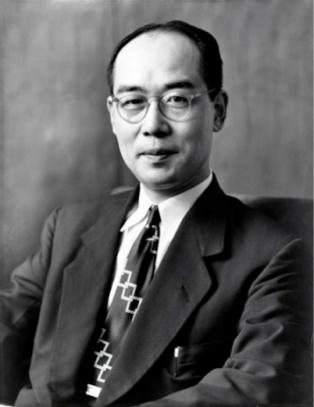
\includegraphics[width=0.2\linewidth]{pics/headshot_yukawa.jpg} \\ \vspace{-.1cm} \hfill \tiny{Hideki Yukawa (1907-1981)}}
\end{frame}
%\fi


% ==============
% Goals Section
% ==============
\section{Goals}

% -----------
% Motivation
% -----------
%\iffalse
\begin{frame}{Why is this important?}
    \begin{itemize}[<+-| alert@+>]
        \item Provides a simple computational model for interactions between nucleons
        \item Allows for visualization for bound and pseudo-bound states
        \item Provides calculation for systems beyond the simple Hydrogen model
        %\item Dr. Wang gave it to me so I did it
        %\item jk (sorta)
    \end{itemize}
\end{frame}
%\fi

% ------
% Goals
% ------
%\iffalse
\begin{frame}{Goals}
    \begin{itemize}[<+-| alert@+>]
        \item Build a solver in Python based on \texttt{hydrogen.py}
        \begin{itemize}
            \item Solve for bound and pseudo-bound states with associated eigenenergies
            \item Produce plots for potential, reduced radial wave function $u_{nl}(r)$, and eigenenergies
            \item Compare results with differing strength and range parameters
        \end{itemize}
    \end{itemize}
\end{frame}
%\fi


% ================
% Methods Section
% ================
\section{Methods}

% -----
% Math
% -----
%\iffalse
\begin{frame}{Mathematics}
    \begin{itemize}[<+-| alert@+>]
        \item Radial Schr\"odinger Equation: \[-\frac{\hbar^2}{2m} \frac{d^2 u}{dr^2} + \bigg[V(r) + \frac{\hbar^2}{2m} \frac{\ell (\ell + 1)}{r^2} \bigg]u = Eu\]
        
        \item Numerov's Method: \[u_{i+1} = \Big(1 + \frac{h^2}{12}f_{i+1} \Big)^{-1} \Big[2 \Big(1 - \frac{5 h^2}{12}f_i \Big)u_i - \Big(1 + \frac{h^2}{6}f_{i-1} \Big)u_{i-1}\Big]\] 
        
        \item Shooting Method: \[f(E) = u_m^\downarrow w_m^\uparrow - u_m^\uparrow w_m^\downarrow, \hspace{.1cm} w = u' \implies w' = u''\]
        
    \end{itemize}
\end{frame}
%\fi

%\iffalse
\begin{frame}{Mathematics}
    \begin{itemize}[<+-| alert@+>]
        \item How can we implement these equations in a simulation?
        \begin{itemize}[<+-| alert@+>]
            \item Introducing... Python!
        \end{itemize}
    \end{itemize}
\end{frame}
%\fi

% ------------
% Computation
% ------------
%\iffalse
\begin{frame}{Computation}
    \begin{itemize}[<+-| alert@+>]
        \item {Use \texttt{hydrogen.py} %\cite{WangCP} 
        source code as foundation}
        \begin{itemize}
            \item $V(r) = 1/r \rightarrow V(r) = e^{-\lambda r}/r$
        \end{itemize}
        \item Packages: NumPy, Matplotlib, SciPy
        \item Define functions for potentials, Numerov method, and shooting method
        \item Calculate energy and approximate wave function in a \texttt{for} loop over initialized $\ell$-values
        \begin{itemize}
            \item \texttt{while} loop nested inside \texttt{for} loop for energy bounds
        \end{itemize}
    \end{itemize}
\end{frame}
%\fi

%\iffalse
\begin{frame}{Numerov Method Function} 
    %\\
        {
        \texttt{def numerov(f, u, n, x, h):} \\
        \hspace{0.5cm} \texttt{nodes, c = 0, h**2/12.} \\
        \hspace{0.5cm} \texttt{f0, f1 = f(x), f(x+h)} \\
        \hspace{0.5cm} \texttt{for i in range(n):} \\
        \hspace{0.5cm} \hspace{0.5cm} \texttt{x += h} \\
        \hspace{0.5cm} \hspace{0.5cm} \texttt{f2 = f(x+h)} \\
        \hspace{0.5cm} \hspace{0.5cm} \texttt{u.append($^*\texttt{insert Numerov equation here}^*$)} \\
        \hspace{0.5cm} \hspace{0.5cm} \texttt{f0, f1 = f1, f2} \\
        \hspace{0.5cm} \hspace{0.5cm} \texttt{if u[-1]*u[-2] < 0.0:} \\
        \hspace{0.5cm} \hspace{0.5cm} \hspace{0.5cm} \texttt{nodes += 1} \\
        \hspace{0.5cm} \texttt{return u, nodes}
        }
\end{frame}
%\fi

%\iffalse
\begin{frame}{Shooting Method Function} 
    %\\
        {
        \texttt{def shoot(En):} \\
        \hspace{0.5cm} \texttt{Global E} \\
        \hspace{0.5cm} \texttt{E, c, xm = En, (h**2)/6., xL + M*h} \\
        \hspace{0.5cm} \texttt{wfup, nup = numerov(f, [0,.1], M, xL, h)} \\
        \hspace{0.5cm} \texttt{wfdn, ndn = numerov(f, [0,.1], N-M, xR, -h)} \\
        \hspace{0.5cm} \texttt{dup = ((1+c*f(xm+h))*wfup[-1] - \\
        \hspace{1.85cm} (1+c*f(xm-h))*wfup[-3])/(h+h)} \\
        \hspace{0.5cm} \texttt{ddn = ((1+c*f(xm+h))*wfdn[-3] - \\
        \hspace{1.85cm} (1+c*f(xm-h))*wfdn[-1])/(h+h)} \\
        \hspace{0.5cm} \texttt{return dup*wfdn[-2] - wfup[-2]*ddn} \\
        }
\end{frame}
%\fi

%\iffalse
\begin{frame}{Example Code}
\begin{columns}
    \begin{column}{0.4\textwidth}
    \large{Bound States:}
        \\
        \vspace{.2cm}
        %\iffalse
        \small{
        \texttt{Lmax, Estart = 4, -V0  %\# declare max L and lower energy bound
        } \\
        \texttt{EL = []} \\
        \texttt{for L in range(Lmax):} \\
        \hspace{0.5cm} \texttt{while Estart < 0:} \\
        \hspace{0.5cm} \hspace{0.5cm} \texttt{E += dE} \\
        \hspace{0.5cm} \hspace{1cm} \texttt{$\cdot$} \\
        \hspace{0.5cm} \hspace{1cm} \texttt{$\cdot$} \\
        \hspace{0.5cm} \hspace{1cm} \texttt{$\cdot$} \\
        \hspace{0.5cm} \hspace{0.5cm} \texttt{print(E, n, l)} \\
        \hspace{0.5cm} \texttt{EL.append(E)} \\
        }
        %\fi

    \end{column}

    \begin{column}{0.58\textwidth}
    \large{Pseudo-Bound States:}
        \\
        \vspace{.2cm}
        %\iffalse
        \small{
        \texttt{Lmax, Estart = 4, -V0} \\
        \texttt{EL = []} \\
        \texttt{for L in range(Lmax):} \\
        \hspace{0.5cm} \texttt{while Estart < exp(-$\lambda$*a)/a:} \\
        \hspace{0.5cm} \hspace{0.5cm} \texttt{E += dE} \\
        \hspace{0.5cm} \hspace{1cm} \texttt{$\cdot$} \\
        \hspace{0.5cm} \hspace{1cm} \texttt{$\cdot$} \\
        \hspace{0.5cm} \hspace{1cm} \texttt{$\cdot$} \\
        \hspace{0.5cm} \hspace{0.5cm} \texttt{print(E, n, l)} \\
        \hspace{0.5cm} \texttt{EL.append(E)} \\
        }
        %\fi
    
    \end{column}
\end{columns}
    
\end{frame}
%\fi


% ===================
% Conclusion Section
% ===================
\section{Results \& Discussion}

% --------
% Results
% --------


% ~~~~~~~~~~
% Potential
% ~~~~~~~~~~
%\iffalse
\begin{frame}{Potential Energy}
    % GS wf & prob density
    \begin{figure}[h]
        \centering
        % Potential for L=0
        \begin{subfigure}{0.45\textwidth}
            \centering
            
\includegraphics[width=\linewidth]{plots/Potential/pb_Vr_L0.pdf}
            \caption{Potential energy $V$ as a function of $r$ for $\ell = 0$.}
        \end{subfigure}
        \hfill
        % Potential for L=1
        \begin{subfigure}{0.45\textwidth}
            \centering
            
\includegraphics[width=\linewidth]{plots/Potential/pb_Vr_L1.pdf}
            \caption{Potential energy $V$ as a function of $r$ for $\ell = 1$.}
        \end{subfigure}
        % Potential for L=5
        \begin{subfigure}{0.45\textwidth}
            \centering
            
\includegraphics[width=\linewidth]{plots/Potential/pb_Vr_L5.pdf}
            \caption{Potential energy $V$ as a function of $r$ for $\ell = 5$.}
        \end{subfigure}
        \caption{}
    \end{figure}
\end{frame}
%\fi

% ~~~~~~~
% Energy
% ~~~~~~~
%\iffalse
\begin{frame}{Energy Plot}
    % Energy Plot/Outputs
    % Energy with Coulomb potential
    \begin{figure}[h]
        \begin{subfigure}{0.45\textwidth}
            \centering
            
\includegraphics[width=\linewidth]{plots/Energy/H_energy.pdf}
            \caption{Eigenenergies for Hydrogen up to $\ell = 5$.}
        \end{subfigure}
        \hfill
        % Energy for Yukawa potential
        \begin{subfigure}{0.45\textwidth}
            \centering
            
\includegraphics[width=\linewidth]{plots/Energy/pb_energy.pdf}
            \caption{Eigenenergies for Yukawa potential up to $\ell = 5$.}
        \end{subfigure}
    \end{figure}
\end{frame}
%\fi

% ~~~~~~~~~~~~~~~~~~~~~
% WFs & prob densities
% ~~~~~~~~~~~~~~~~~~~~~
%\iffalse
\begin{frame}{Wave Functions \& Probability Densities}
    % GS wf & prob density
    \begin{figure}[h]
        \centering
        % WF for u_10
        \begin{subfigure}{0.45\textwidth}
            \centering
            
\includegraphics[width=\linewidth]{plots/WFs&PDs/pb_wf_u10.pdf}
            \caption{Reduced radial wave function $u_{10}$ as a function of $r$.}
        \end{subfigure}
        \hfill
        % Prob density for u_10
        \begin{subfigure}{0.45\textwidth}
            \centering
            
\includegraphics[width=\linewidth]{plots/WFs&PDs/pb_pd_u10.pdf}
            \caption{Probability density for $u_{10}$ as a function of $r$.}
        \end{subfigure}
        % Energy for u_10
        \begin{subfigure}{0.45\textwidth}
            \centering
            
\includegraphics[width=\linewidth]{plots/Energy/pb_pot_E10.pdf}
            \caption{Ground state energy $E_{10}$ and potential as a function of $r$.}
        \end{subfigure}
        \caption{}
    \end{figure}
\end{frame}
%\fi

%\iffalse
\begin{frame}{Wave Functions \& Probability Densities}
    % n=7, L=5 wf & prob density
    \begin{figure}[h]
        \centering
        % WF for u_75
        \begin{subfigure}{0.45\textwidth}
            \centering
            
\includegraphics[width=\linewidth]{plots/WFs&PDs/pb_wf_u75.pdf}
            \caption{Reduced radial wave function $u_{75}$ as a function of $r$.}
        \end{subfigure}
        \hfill
        % Prob density for u_75
        \begin{subfigure}{0.45\textwidth}
            \centering
            
\includegraphics[width=\linewidth]{plots/WFs&PDs/pb_pd_u75.pdf}
            \caption{Probability density for $u_{75}$ as a function of $r$.}
        \end{subfigure}
        % Energy for u_75
        \begin{subfigure}{0.45\textwidth}
            \centering
            
\includegraphics[width=\linewidth]{plots/Energy/pb_pot_E75.pdf}
            \caption{Energy $E_{75}$ and $V_{\text{eff}}$ as a function of $r$.}
        \end{subfigure}
        \caption{}
    \end{figure}
\end{frame}
%\fi

%\iffalse
\begin{frame}{Wave Functions \& Probability Densities}
    % n=6, L=3 wf & prob density
    \begin{figure}[h]
        \centering
        % WF for u_63
        \begin{subfigure}{0.45\textwidth}
            \centering
            
\includegraphics[width=\linewidth]{plots/WFs&PDs/pb_wf_u63.pdf}
            \caption{Reduced radial wave function $u_{63}$ as a function of $r$.}
        \end{subfigure}
        \hfill
        % Prob density for u_63
        \begin{subfigure}{0.45\textwidth}
            \centering
            
\includegraphics[width=\linewidth]{plots/WFs&PDs/pb_pd_u63.pdf}
            \caption{Probability density for $u_{63}$ as a function of $r$.}
        \end{subfigure}
        % Energy for u_10
        \begin{subfigure}{0.45\textwidth}
            \centering
            
\includegraphics[width=\linewidth]{plots/Energy/pb_pot_E63.pdf}
            \caption{Energy $E_{63}$ and potential as a function of $r$.}
        \end{subfigure}
        \caption{}
    \end{figure}
\end{frame}
%\fi

%\iffalse
\begin{frame}{Wave Functions \& Probability Densities}
    % n=6, L=3 wf & prob density
    \begin{figure}[h]
        \centering
        % WF for u_63
        \begin{subfigure}{0.45\textwidth}
            \centering
            
\includegraphics[width=\linewidth]{plots/WFs&PDs/pb_wf_u255.pdf}
            \caption{Reduced radial wave function $u_{25,5}$ as a function of $r$.}
        \end{subfigure}
        \hfill
        % Prob density for u_63
        \begin{subfigure}{0.45\textwidth}
            \centering
            
\includegraphics[width=\linewidth]{plots/WFs&PDs/pb_pd_u255.pdf}
            \caption{Probability density for $u_{25,5}$ as a function of $r$.}
        \end{subfigure}
        % Energy for u_10
        \begin{subfigure}{0.45\textwidth}
            \centering
            
\includegraphics[width=\linewidth]{plots/Energy/pb_pot_E255.pdf}
            \caption{Energy $E_{25,5}$ and potential as a function of $r$.}
        \end{subfigure}
        \caption{}
    \end{figure}
\end{frame}
%\fi


% -----------
% Discussion
% -----------
%\iffalse
\begin{frame}{Discussion}
    \begin{itemize}[<+-| alert@+>]
        \item What does this data mean?
        \begin{itemize}
            \item A computational model with the piecewise Yukawa potential is feasible
            \item As $a$ increases, more bound states appear
            \item As $V_0$ increases, more bound states appear
            \item As $\lambda$ increases, what happens?
        \end{itemize}
    \end{itemize}
\end{frame}
%\fi


% ===============
% Moving Forward
% ===============
\section{Moving Forward}

% --------------
% Going Forward
% --------------
%\iffalse
\begin{frame}{Moving Forward}
    \begin{itemize}[<+-| alert@+>]
        \item Calculate tunneling probability for pseudo-bound and scattering states
        \item Determine at which well depth/width bound states start to appear
        \item Continue to push the limits of $\lambda$ to draw a more determined conclusion from its effects
    \end{itemize}
\end{frame}
%\fi


% ===========
% AI Section
% ===========
\section{AI Implementation}

% -------
% AI Use
% -------
%\iffalse
\begin{frame}{AI Implementation}
    \begin{itemize}[<+-| alert@+>]
        \item Clarifying analysis of reference material
        \item Code production, comparison, and debugging
        \item Document formatting
    \end{itemize}
\end{frame}
%\fi


% ================
% Reference Slide
% ================
\section{References}

% -------------
% References 1
% -------------
%\iffalse
\begin{frame}{References}
    \begin{thebibliography}{9}
    \vspace{-.2cm}
        % Griffiths QM [1]
        \bibitem{GriffithsQM}{D. J. Griffiths, {\em Introduction to Quantum Mechanics}, 2nd ed. (Pearson Prentice Hall, 2005).}

        % Wang Comp. Physics (2016) [2]
        \bibitem{WangCP}{J. J. Wang, {\em Computational Modeling and Visualization of Physical Systems with Python}, (Wiley, 2016), Chap. 9.}

        % Yukawa Original Paper [3]
        \bibitem{Yukawa1935}{H. Yukawa, ``On the Interaction of Elementary Particles,'' {\em Proc. Phys.-Math. Soc. Japan} {\bf 17}, 48--57 (1935).}

        % Yukawa Memorial Cite (Yukawa Picture) [4]
        \bibitem{YukMem}{Yukawa Memorial, The University of Osaka, ``About Hideki Yukawa,'' {\em The University of Osaka}. Available at: \url{https://www-yukawa.phys.sci.osaka-u.ac.jp/en/yukawahideki}%(accessed May 2, 2026)
        .}
    \end{thebibliography}
\end{frame}
%\fi

% -------------
% References 2
% -------------
\iffalse
\begin{frame}{References}
    \begin{thebibliography}{9}
        % ChatGPT [5]
        \bibitem{ChatGPT} OpenAI (2026). \textit{ChatGPT} [Large language model]. \url{https://chat.openai.com/}

        % Gemini [6]
        \bibitem{GeminiAI} Google (2026). \textit{Gemini} [Large language model]. \url{https://gemini.google.com/}

    \end{thebibliography}
\end{frame}
\fi

\end{document}  